\iffalse
\documentclass[12pt]{article}
\usepackage{graphicx}
%\documentclass[journal,12pt,twocolumn]{IEEEtran}
\usepackage[none]{hyphenat}
\usepackage{graphicx}
\usepackage{listings}
\usepackage[english]{babel}
\usepackage{graphicx}
\usepackage{caption} 
\usepackage{hyperref}
\usepackage{booktabs}
\def\inputGnumericTable{}
\usepackage{color}                                            %%
    \usepackage{array}                                            %%
    \usepackage{longtable}                                        %%
    \usepackage{calc}                                             %%
    \usepackage{multirow}                                         %%
    \usepackage{hhline}                                           %%
    \usepackage{ifthen}
\usepackage{array}
\usepackage{amsmath}   % for having text in math mode
\usepackage{listings}
\lstset{
language=tex,
frame=single, 
breaklines=true
}
  
%Following 2 lines were added to remove the blank page at the beginning
\usepackage{atbegshi}% http://ctan.org/pkg/atbegshi
\AtBeginDocument{\AtBeginShipoutNext{\AtBeginShipoutDiscard}}
%


%New macro definitions
\newcommand{\mydet}[1]{\ensuremath{\begin{vmatrix}#1\end{vmatrix}}}
\providecommand{\brak}[1]{\ensuremath{\left(#1\right)}}
\providecommand{\norm}[1]{\left\lVert#1\right\rVert}
\newcommand{\solution}{\noindent \textbf{Solution: }}
\newcommand{\myvec}[1]{\ensuremath{\begin{pmatrix}#1\end{pmatrix}}}
\let\vec\mathbf

\begin{document}

\begin{center}
\title{\textbf{Coordinate Geometry}}
\date{\vspace{-5ex}} %Not to print date automatically
\maketitle
\end{center}

\setcounter{page}{1}



\begin{enumerate}

\item\textbf{Problem statement :} Find a relation between x and y such that the point $\myvec{x ,y}$ is equidistant from the point $\myvec{3 ,6}$ and $\myvec{-3 ,4}$

\solution \\
\textbf{\centering{Method I}}
\fi
The input parameters for this problem are given as
	\begin{align}
	\vec{P} = \myvec{
		x\\
		y\\
		},
	\vec{A} = \myvec{
		3\\
		6\\
		},
        \vec{B} = \myvec{
		3\\
		-4\\
		}
	\end{align}
\iffalse

  If $\vec{P}$ equidistant from the points $\vec{A}$ and $\vec{B}$, 
\begin{align}
 \norm{\vec{P}-\vec{A}} &=
\norm{\vec{P}-\vec{B}} 
\\
 \implies \norm{\vec{P}-\vec{A}}^2 &=
\norm{\vec{P}-\vec{B}}^2 
\end{align}
which can be expressed as 
\begin{align}
%  \label{eq:chapters/10/7/1/10/norm2d_dist}
 \brak{\vec{P}-\vec{A}}^{\top} \brak{\vec{P}-\vec{A}}=
 \brak{\vec{P}-\vec{B}}^{\top} 
\brak{\vec{P}-\vec{B}}
\\
 \implies \norm{\vec{P}}^2-2{\vec{P}}^{\top}\vec{A} + \norm{\vec{A}}^2
 \\= \norm{\vec{P}}^2-2{\vec{P}}^{\top}\vec{B} + \norm{\vec{B}}^2
\end{align}
which can be simplified to obtain
%  \eqref{eq:chapters/10/7/1/10/norm2d_equidist}.
  \fi
  \begin{align}
   \vec{P} =
    y\vec{e}_1
  \end{align}
  where 
  \begin{align}
   y &=\frac{\norm{\vec{A}}^2 -\norm{\vec{B}}^2 }{2\brak{\vec{A}-\vec{B}}^{\top }\vec{e}_1
}\label{eq:chapters/10/7/1/10/5}  
  \end{align}
  Substituting the $\vec{A}, \vec{B}$ values in \eqref{eq:chapters/10/7/1/10/5},
\begin{align}
 \brak{\vec{A}-\vec{B}}=
 \myvec{6 \\ 2},
   \norm{\vec{A}}^2 = 45,
   \norm{\vec{B}}^2 = 25
    \end{align}
    yielding
$y =  5$.
Hence, 
\begin{align}
\vec{P} = \myvec{ 0 \\ 5}
\end{align}
%
See Fig. 
\ref{fig:chapters/10/7/1/10/Fig1}.
\begin{figure}[!h]
 \begin{center}
  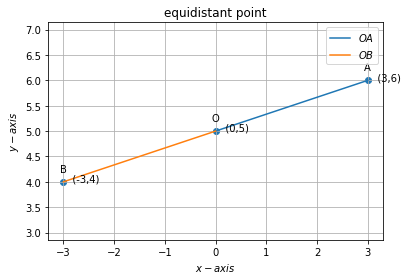
\includegraphics[width=\columnwidth]{./chapters/10/7/1/10/figs/fig.png}
 \end{center}
\caption{}
\label{fig:chapters/10/7/1/10/Fig1}
\end{figure}

